\section{Árboles de decisión}

Los árboles de decisión son modelos de predicción utilizados en inteligencia artificial que toma como entrada un conjunto de atributos y devuelve un valor que representa la decisión tomada por el árbol, este valor puede ser discreto o continuo. Los nodos internos del árbol contienen un test sobre una o varios atributos de entrada, según el resultado del test así será el camino que se sigue hasta llegar a una hoja, en las hojas se encuentran las posibles decisiones que el árbol puede tomar\cite{B4}.

Como los árboles de decisión son muy aplicados en problemas de clasificación, vamos a utilizar esta técnica para la clasificación de aquellas noticias de las que desconocemos su categoría. Para la experimentación hemos utilizado la herramienta WEKA y la implementación del algoritmo C4.5 que incluye.

\subsection{Algoritmo C4.5}
El algotirmo C4.5 es un algoritmo propuesto por Quinlan basado en un algoritmo anterior llamado ID3. El C4.5 genera árboles de decisión que tiene como objetivo determinar la clase $(C_{1},C_{2},...C_{x})$ a la que pertenece un objeto a partir de la evaluación de un conjunto de atributos, su uso está bastante extendido en las áreas de aprendizaje automático y minería de datos\cite{B1}. 

El árbol de decisión se genera a partir de un set de entrenamiento, este set contiene un conjunto de ejemplos ya clasificados $S = (s_{1},s_{2},...s_{n})$ y cada ejemplo $s_{n}$, está formado por un conjunto de atributos $(d_{1},d_{2},...d_{n})$ y una clase $C_{x}$. El árbol se compone de nodos de decisión y hojas, en los nodos de decisión se toma un atributo y se realiza un test sobre él, para el caso de atributos continuos este test determina un valor de umbral t para tomar una decisión en función de dos posibilidades, que son $d_{n} \leq t$ o $d_{n} \textgreater t$. Las hojas del árbol se corresponden con alguna clase.

El árbol generado se aplica en problemas de clasificación, basándonos en los valores de los atributos vamos construyendo un camino desde la raíz del árbol hasta alguna hoja, la clase que contiene la hoja a la que se llega será la clase que sugiera el algoritmo como clase de un ejemplo sin clasificar.


\subsubsection{Determinar la calidad del árbol}
Para determinar la bondad del clasificador obtenido se mide la cantidad de ejemplos que se han clasificado de forma correcta. Esta valoración se suele dar en tanto por ciento y se calcula a partir de dos parámetros que son el número de ejemplos correctamente clasificados (True Positive Rate) y los clasificados incorrectamente (False Positive Rate). 

Con los datos anteriores también se puede crear un matriz de confusión, esta matriz cuadrada de tamaño $n$, donde $n$ es el número de clases y contiene el número de elementos clasificados de forma correcta e incorrecta. Las columnas contienen las clases que predice el algoritmo y las filas las propias clases de forma que la diagonal de la matriz contiene los ejemplos correctamente clasificados y el resto de celdas contiene errores. La ventaja de usar esta matriz es que permite visualizar de forma rápida si una o varias clases se están clasificando de forma errónea. \cite{B3}
\subsection{Creación del conjunto de datos}

Un conjunto de datos de weka tiene la estructura que se puede ver en el siguiente bloque de texto, los elementos principales son los atributos (\textit{@attribute}) y los datos (\textit{@data}).

Para la realización de experimentos de clasificación con Weka necesitamos definir lo que son atributos y datos, para la selección de atributos tenemos un conjunto de valores numéricos, cada valor representa una palabra tomada del conjunto de palabras seleccionado con el procedimiento descrito en la sección \nameref{sec:atributos} y un atributo extra que representa las distintas clases que tenemos, estas clases es nuestro conjunto de categorías. 

Para generar la parte de datos se han tomado dos aproximaciones. La primera es crear un conjunto de datos donde el valor de cada atributo es la frecuencia media con la que aparece la palabra dentro de la categoría a la que pertenece la noticia, la segunda es una aproximación booleana donde solo se tiene en cuenta si la palabra aparece o no en la noticia.

A continuación se muestra un fragmento de uno de los conjuntos de datos que hemos creado:
\begin{lstlisting}
@relation Semandal

@attribute @@class@@ {Agricultura,Comercio,cultura,Cursos,Deportes,economia,Educacion...}
@attribute sector numeric
@attribute cobre numeric
@attribute cultura numeric
@attribute sociales numeric
@attribute agricultura numeric
@attribute empleo numeric
	.
	.
	.
	.		
@attribute seguridad numeric
@attribute actividades numeric

@data
turismo1, 0, 0, 0, 0, 0, 0, ... 0, 0
ssociales, 0, 0, 0, 0.545905707196, 0, ... 0, 0
recursosHumanos, 0, 0, 0, 0, 0, 0, ... 0, 0
obras, 0, 0, 0, 0, 0, 0, ... 0, 0, 0
igualdad, 0, 0, 0, 0, 0, ... 0, 0
Mujer, 0, 0, 0, 0, 0, 0, ... 0, 0
PIM, 0, 0, 0, 0, 0, 0, ... 0, 0
consumo, 0, 0, 0, 0, 0, 0, ... 0, 0
\end{lstlisting}
\subsubsection{Conjunto de datos con frecuencia de apariciones}

Para crear la sección de atributos, primero hemos calculado el conjunto de palabras característico de cada categoría obteniendo una lista de palabras junto con su relevancia dentro de la categoría, siguiendo el procedimiento descrito en \nameref{sec:atributos}. A continuación se han concatenado las listas de todas las categorías eliminando repetidos, esta nueva lista de atributos incluye palabras como \textit{agricultura, cobre, cultura, empleo, etc}, son las palabras que se pueden ver en el conjunto de datos anterior en la parte de \textit{@attribute}.

Luego hemos tomado un número de noticias por categoría, cada texto se corresponderá con un registro del conjunto de datos (\textit{@data}), a continuación se muestra un posible ejemplo:


\glqq El Ayuntamiento de Punta Umbría, con la colaboración de los centros de Primaria de la localidad, ha organizado un certamen de dibujo para escolares bajo el título 'El agua es vida'. El concejal delegado de Medio Ambiente del Consistorio costero, Andrés Franco Ramos, repartirá mañana miércoles, 25 de marzo, los premios a los mejores trabajos de cada colegio puntaumbrieño. Así, a las 13.00 horas está previsto que acuda al CEIP Virgen del Carmen.

Con este concurso el Consistorio costero conmemoró el Día Mundial del Agua, que se celebró el pasado 22 de marzo \grqq

Para crear una línea del conjunto de datos en la sección \textit{@data}, lo primero buscar la categoría de la noticia, esta categoría se corresponde con uno de los posibles valores del atributo \textit{@@class@@}. A continuación debemos apuntar \textit{n} elementos, uno por cada palabra de la lista de atributos. Para determinar el valor que hay que anotar debemos ver si cada palabra de la lista de atributos aparece en la noticia. Si no se encuentra la palabra en la noticia, en el conjunto de datos escribimos el valor cero. Si la palabra aparece en la noticia, buscamos el valor de frecuencia de apariciones de la palabra dentro de la categoría de la noticia y anotamos el valor correspondiente. Si la palabra no es relevante dentro de la categoría de la noticia, aunque se encuentre en la lista de atributos y en la noticia, escribimos un cero. El resultado de este proceso es cada una de las líneas que se puede ver en el conjunto de datos anterior en la sección \textit{@data}.

\subsubsection{Conjunto de datos booleano}

Una segunda aproximación es crear un conjunto de datos donde solo habrá dos posibles valores para los atributos, 1 si la palabra aparece en la noticia o 0 si la palabra no está en la noticia. El método de construcción de este conjunto de datos es el mismo que hemos utilizado en el caso anterior, pero anotando uno de los dos valores anteriores en vez de la frecuencia con la que aparece la palabra.

\subsection{Experimentación}
\subsubsection{Pruebas realizadas}
Para las pruebas hemos realizado un conjunto de datos para la herramienta WEKA, para ver la relación entre el tamaño del conjunto de datos y la precisión del clasificador resultante hemos probado distintos tamaños de conjunto de datos que se detallan a continuación:
\vspace{1em}
\begin{center}
\begin{tabular}{|c|c|c|}
\hline 
Experimentos & Número de palabras & Número de noticias \\ 
\hline 
Experimento 1 & 1064 & 2842 \\ 
\hline 
Experimento 2 & 1649 & 4478 \\ 
\hline 
Experimento 3 & 2124 & 5253 \\ 
\hline 
\end{tabular} 
\end{center}
\vspace{1em}
Como algoritmo hemos utilizado PART en WEKA con un cross-validation de 10 folds para el experimento uno y 15 folds para los experimentos dos y tres.
\subsection{Resultados obtenidos}
\label{subsec:resj48}
\subsubsection{Frecuencia de términos}
Los resultados obtenidos muestran una mejora de la precisión del clasificador obtenido conforme se aumenta el tamaño del conjunto de datos, aunque son sucesivos aumentos del conjunto de datos la mejora es cada vez menor. Las tasas de aciertos obtenidas son las siguientes:
\vspace{1em}
\begin{center}
\begin{tabular}{|c|c|c|c|}
\hline 
- & Experimento 1 & Experimento 2 & Experimento 3 \\ 
\hline 
Tasa de acierto & 56.4391\% & 64.9397\% & 64.6868\% \\ 
\hline 
\end{tabular} 
\end{center}
\vspace{1em}
Seria posible seguir aumentando el tamaño del conjunto de datos pero cada vez la mejora entre experimentos es menor.
Para dar una representación visual de la calidad del clasificador utilizamos matrices de confusión.Las matrices obtenidas son las siguientes:

Experimento 1
\begin{center}
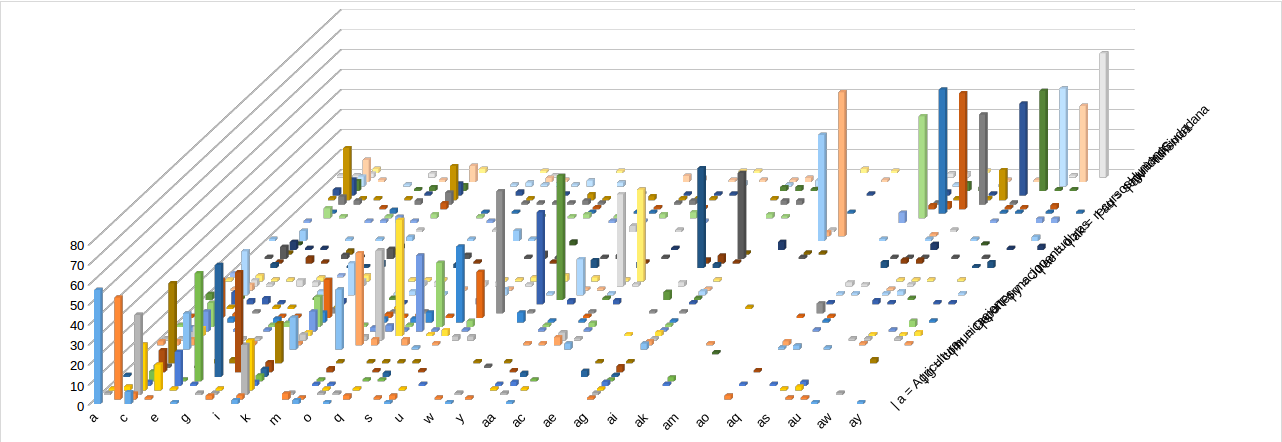
\includegraphics[width=\textwidth]{j48/PART_80_CV10.png} 
\end{center}

Experimento 2
\begin{center}
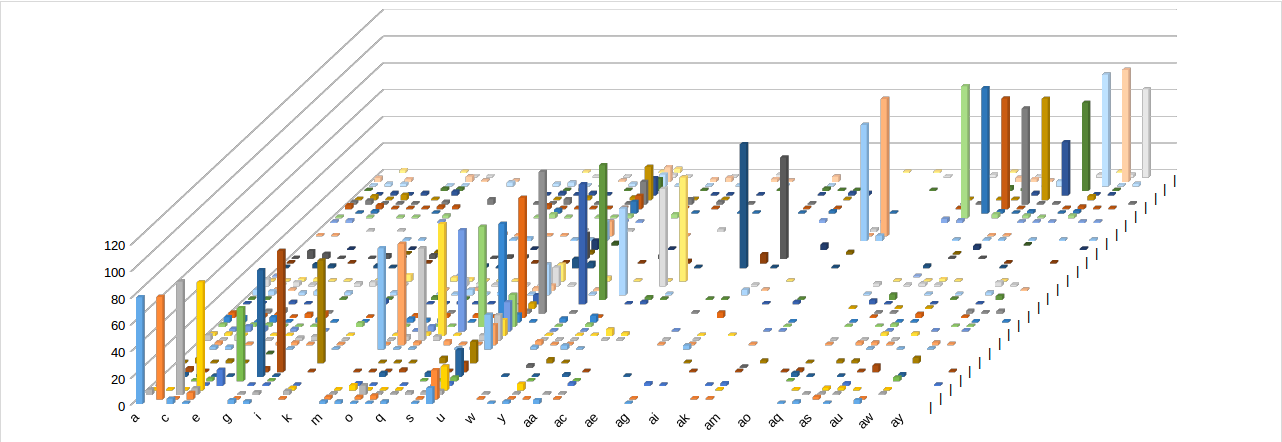
\includegraphics[width=\textwidth]{j48/PART_125_CV15.png} 
\end{center}

Experimento 3
\begin{center}
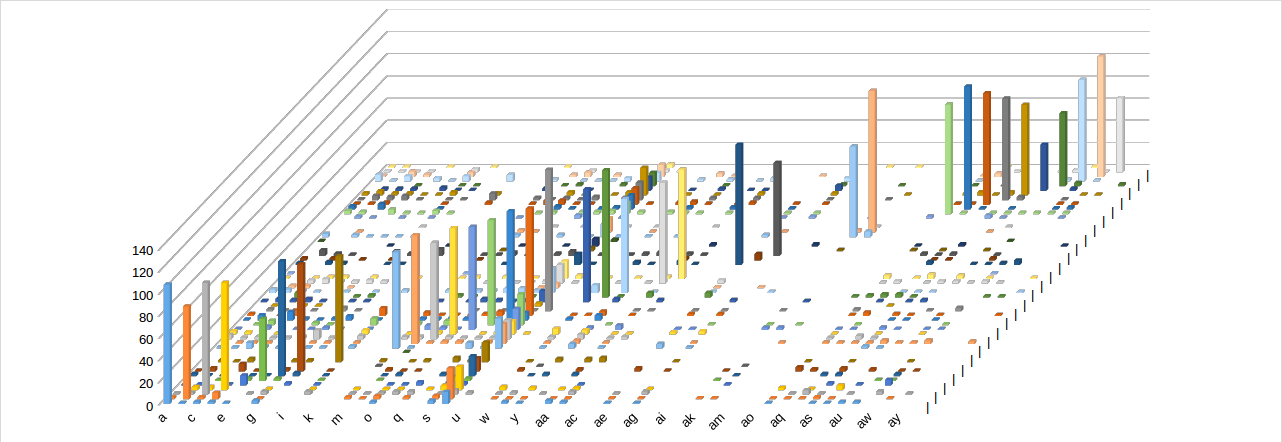
\includegraphics[width=\textwidth]{j48/PART_175_CV15.png} 
\end{center}
Como se puede observar en el primer experimento el clasificador es capaz de etiquetar correctamente la mayoría de los casos. Solo muestra clasificaciones erróneas con las noticias de las categorías \textit{Ayuntamiento} y  \textit{Cultura}, posiblemente por compartir un gran número de palabras clave con otras categorías. En los siguientes experimentos, al ampliar el conjunto de palabras que determinan cada categoría y el número de ejemplos que se dan al algoritmo, se mejora la clasificación de estas categorías, pero empeora la clasificación de la categoría \textit{Generales}. Esta categoría es una fuente de ruido pues muchos municipios la utilizan sobre noticias que podrían considerarse de otras categorías y hace que la lista de palabras que definen la categoría \textit{Generales} tome palabras de otras categorías que realmente no aportan información dentro de la categoría \textit{Generales}.
\subsubsection{Conjunto de datos Booleanos}

Como en el caso anterior, la precisión aumenta si aumentamos el tamaño del conjunto de datos, pero como se muestra a continuación los resultados son bastante peores que los obtenidos utilizando frecuencia de terminos.
\vspace{1em}
\begin{center}
\begin{tabular}{|c|c|c|c|}
\hline 
- & Experimento 1 & Experimento 2 & Experimento 3 \\ 
\hline 
Tasa de acierto & 28.0185\% & 29.1871\% & 29.209\% \\ 
\hline 
\end{tabular} 
\end{center}
\vspace{1em}
Las matrices de confusión obtenidas son las siguientes:

Experimento 1
\begin{center}
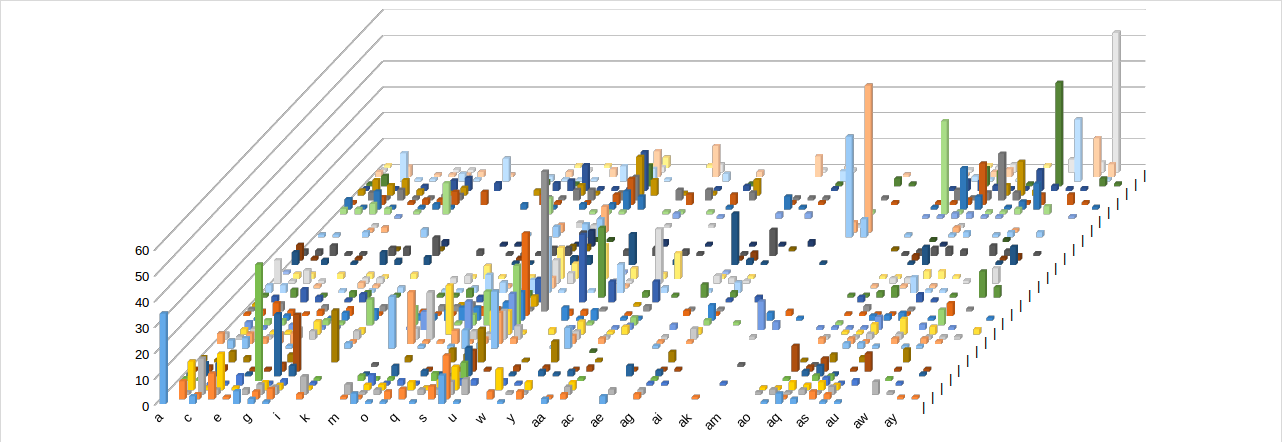
\includegraphics[width=\textwidth]{j48/dataset80_bool.png} 
\end{center}
Experimento 2
\begin{center}
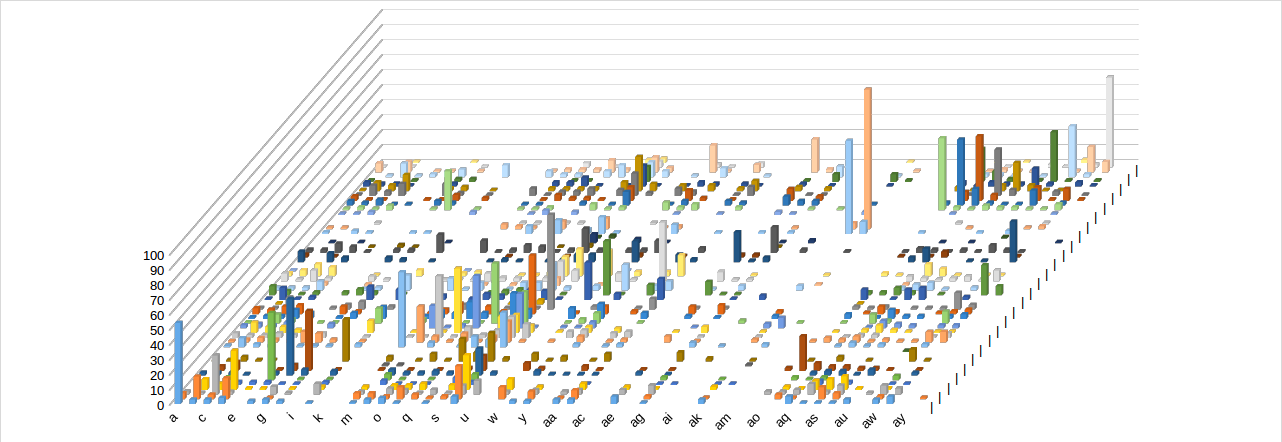
\includegraphics[width=\textwidth]{j48/dataset125_bool.png} 
\end{center}
Experimento 3
\begin{center}
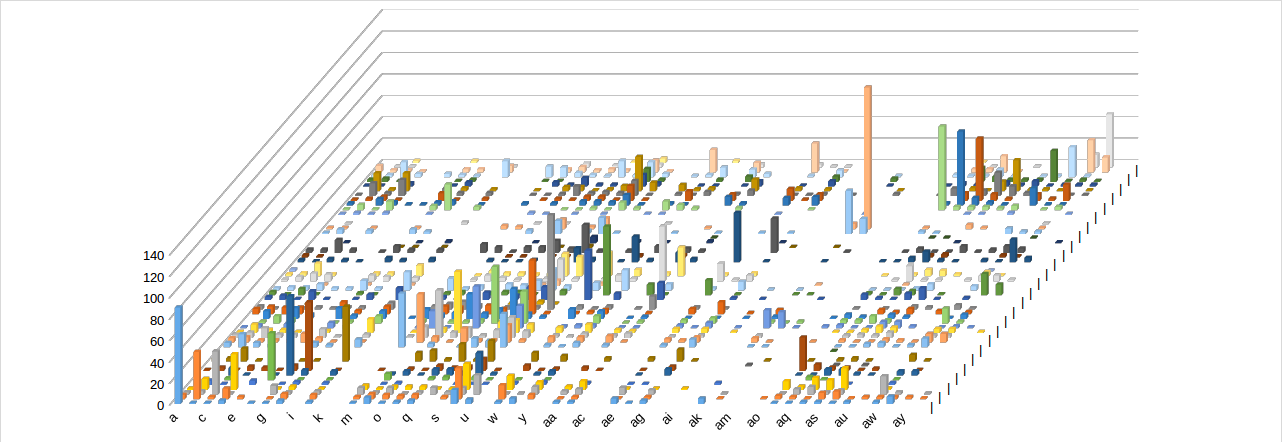
\includegraphics[width=\textwidth]{j48/dataset175_bool.png} 
\end{center}

A la vista de las matrices de confusión obtenidas podemos ver como esta aproximación obtiene unos resultados peores. La razón para esta diferencia en la precisión es que no se tiene en cuenta que el número de textos en cada categoría  no es igual y que una palabra, aunque se utilice en varias categorías, no tiene la misma relevancia en todas ellas.

\subsection{Extracción de reglas}

Para extraer las reglas hemos utilizado la opción PART de WEKA que ejecuta el  algoritmo C4.5 y se utiliza la estrategia divide y vencerás y tecnicas de poda para crear árboles parciales de los cuales extraer reglas hasta cubrir todas las hojas.\cite{A1}\cite{M1}

Una vez obtenidas las reglas en Weka, hemos tomado un código Java escrito por Gonzalo Aranda para cargar las reglas en memoria, modificando el código para leer las reglas en el formato que da Weka, y generar un fichero con las mismas reglas en un formato compatible con CLIPS. Este nuevo fichero se utilizará durante la fase de clasificación.
 
